\begin{table}[ht]
\caption{Complete confirmation policy census. Success uses every planned task. Firing is over eligible prefixes; recoveries and disruptions count the two draw-level comparisons with continuation.}
\label{tab:confirmation-policies}
\centering
\small
\begin{tabular}{@{}llrrrr@{}}
\toprule
Domain & Policy & Success (\%) & Fire (\%) & Recover & Disrupt \\
\midrule
\multirow{6}{*}{ALFWorld} & Continue & 52.86 & 0.0 & 0 & 0 \\
 & Best fixed & 55.34 & 100.0 & 74 & 55 \\
 & Direct & 54.43 & 31.0 & 26 & 14 \\
 & Arm outcome & 54.04 & 96.6 & 69 & 60 \\
 & Matched & 54.82 & 78.0 & 66 & 51 \\
 & Safe selected & 54.82 & 78.0 & 66 & 51 \\
\midrule
\multirow{6}{*}{ScienceWorld} & Continue & 19.30 & 0.0 & 0 & 0 \\
 & Best fixed & 19.30 & 100.0 & 5 & 5 \\
 & Direct & 19.30 & 11.8 & 0 & 0 \\
 & Arm outcome & 19.30 & 100.0 & 5 & 5 \\
 & Matched & 14.04 & 100.0 & 2 & 8 \\
 & Safe selected & 14.04 & 100.0 & 2 & 8 \\
\bottomrule
\end{tabular}
\end{table}

Figure~\ref{fig:effects} shows both marginal task and grouped uncertainty for the primary family and the selected deployment rule. The group intervals are wider whenever shared floorplans induce material composition sensitivity. Statistical significance is determined only by the frozen group sign-flip family, not by whether a plotted interval excludes zero.

\begin{figure}[ht]
\centering
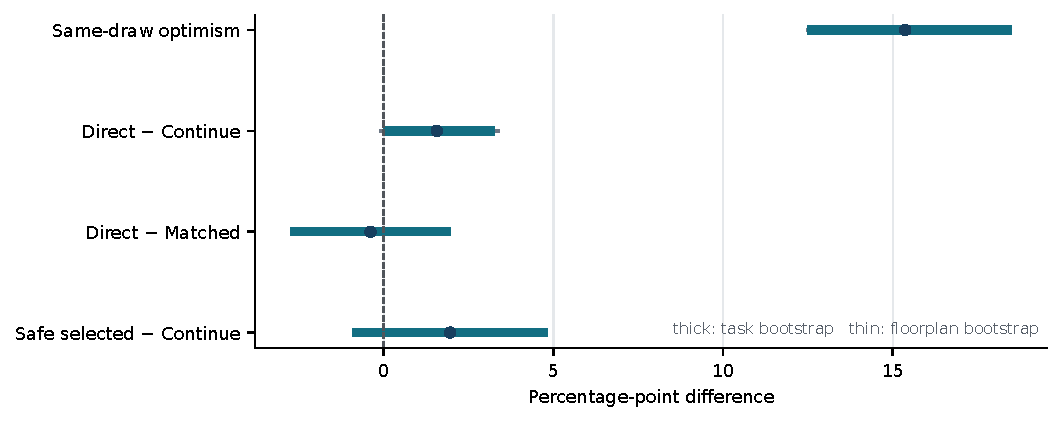
\includegraphics[width=\linewidth]{figures/policy-effects.pdf}
\caption{Confirmation effects on ALFWorld. Dots show planned-task means; thick and thin intervals show task- and floorplan-bootstrap 95\% intervals. Reported adjusted $p$ values use the prespecified group sign-flip tests and Holm correction.}
\label{fig:effects}
\end{figure}
